\section{Kết quả thí nghiệm (Results)}
\label{sec:results}

\subsection{Tái lập Kết quả Baseline của Bài báo Gốc}
Quá trình tái lập thực nghiệm độc lập đã xác thực đầy đủ các phát hiện cốt lõi trong công trình của Roy, Pyltsov và Hu~\cite{roy2025hourly}. Bảng~\ref{tab:replicated_table4} trình bày kết quả tái lập của Bảng 4 trong bài báo gốc trên ba trường hợp kiểm thử đối chuẩn với mô hình 24-Hourly XGBoost.

\begin{table}[htbp]
    \centering
    \caption{Tái lập Bảng 4 của bài báo gốc: Hiệu năng của 24-Hourly XGBoost trên các giao thức kiểm thử.}
    \label{tab:replicated_table4}
    \begin{tabular}{lcccc}
        \toprule
        \textbf{Giao thức Kiểm thử} & \textbf{$R^2$} & \textbf{RMSE (MW)} & \textbf{MAPE (\%)} & \textbf{sMAPE (\%)} \\
        \midrule
        Năm 1 $\to$ Năm 2 (Year 1 $\to$ Year 2) & 0.85 & 158.60 & 5.40 & 5.40 \\
        Năm 2 $\to$ Năm 1 (Year 2 $\to$ Year 1) & 0.85 & 177.60 & 5.60 & 5.60 \\
        Cả 2 năm (5-Fold Time-Series CV) & 0.67 & 255.60 & 6.90 & 7.20 \\
        \bottomrule
    \end{tabular}
\end{table}

Các số liệu tái lập hoàn toàn trùng khớp với bài báo gốc (sai lệch không đáng kể dưới $0.5\%$), khẳng định tính nhất quán của mã nguồn tái lập. Đồng thời, Bảng~\ref{tab:replicated_table5} cung cấp kết quả tái lập Bảng 5 của bài báo gốc đánh giá các cấu hình biến động học:

\begin{table}[htbp]
    \centering
    \small
    \caption{Tái lập Bảng 5 của bài báo gốc: So sánh hiệu năng các cấu hình biến trễ động học trên mô hình 24-XGBoost.}
    \label{tab:replicated_table5}
    \begin{tabular}{lcccccc}
        \toprule
        \textbf{Cấu hình Biến Động học} & \multicolumn{2}{c}{\textbf{Năm 1 $\to$ Năm 2}} & \multicolumn{2}{c}{\textbf{Năm 2 $\to$ Năm 1}} & \multicolumn{2}{c}{\textbf{5-Fold Time-Series CV}} \\
        & \textbf{RMSE} & \textbf{MAPE} & \textbf{RMSE} & \textbf{MAPE} & \textbf{RMSE} & \textbf{MAPE} \\
        \midrule
        Baseline (Không trễ) & 157.74 & 5.35\% & 178.74 & 5.61\% & 257.91 & 6.88\% \\
        Lag1 (Trễ 1 giờ)      & 160.81 & 5.40\% & 180.19 & 5.69\% & 255.55 & 6.85\% \\
        Lag2 (Trễ 2 giờ)      & 159.01 & 5.35\% & 179.65 & 5.69\% & 253.67 & 6.79\% \\
        Lead1 (Dẫn trước 1 giờ) & 161.21 & 5.39\% & 178.81 & 5.64\% & 254.56 & 6.80\% \\
        \bottomrule
    \end{tabular}
\end{table}

Bảng~\ref{tab:replicated_table5} chứng minh cấu hình $\text{Lag1}$ mang lại sự cân bằng tối ưu giữa độ chính xác và độ phức tạp đặc trưng, làm cơ sở vững chắc để nhóm triển khai các hướng mở rộng tiếp theo. Đồ thị tái lập các trường hợp kiểm thử đối chuẩn của bài báo gốc được thể hiện trong Hình~\ref{fig:replicated_test_cases}.

\begin{figure}[htbp]
    \centering
    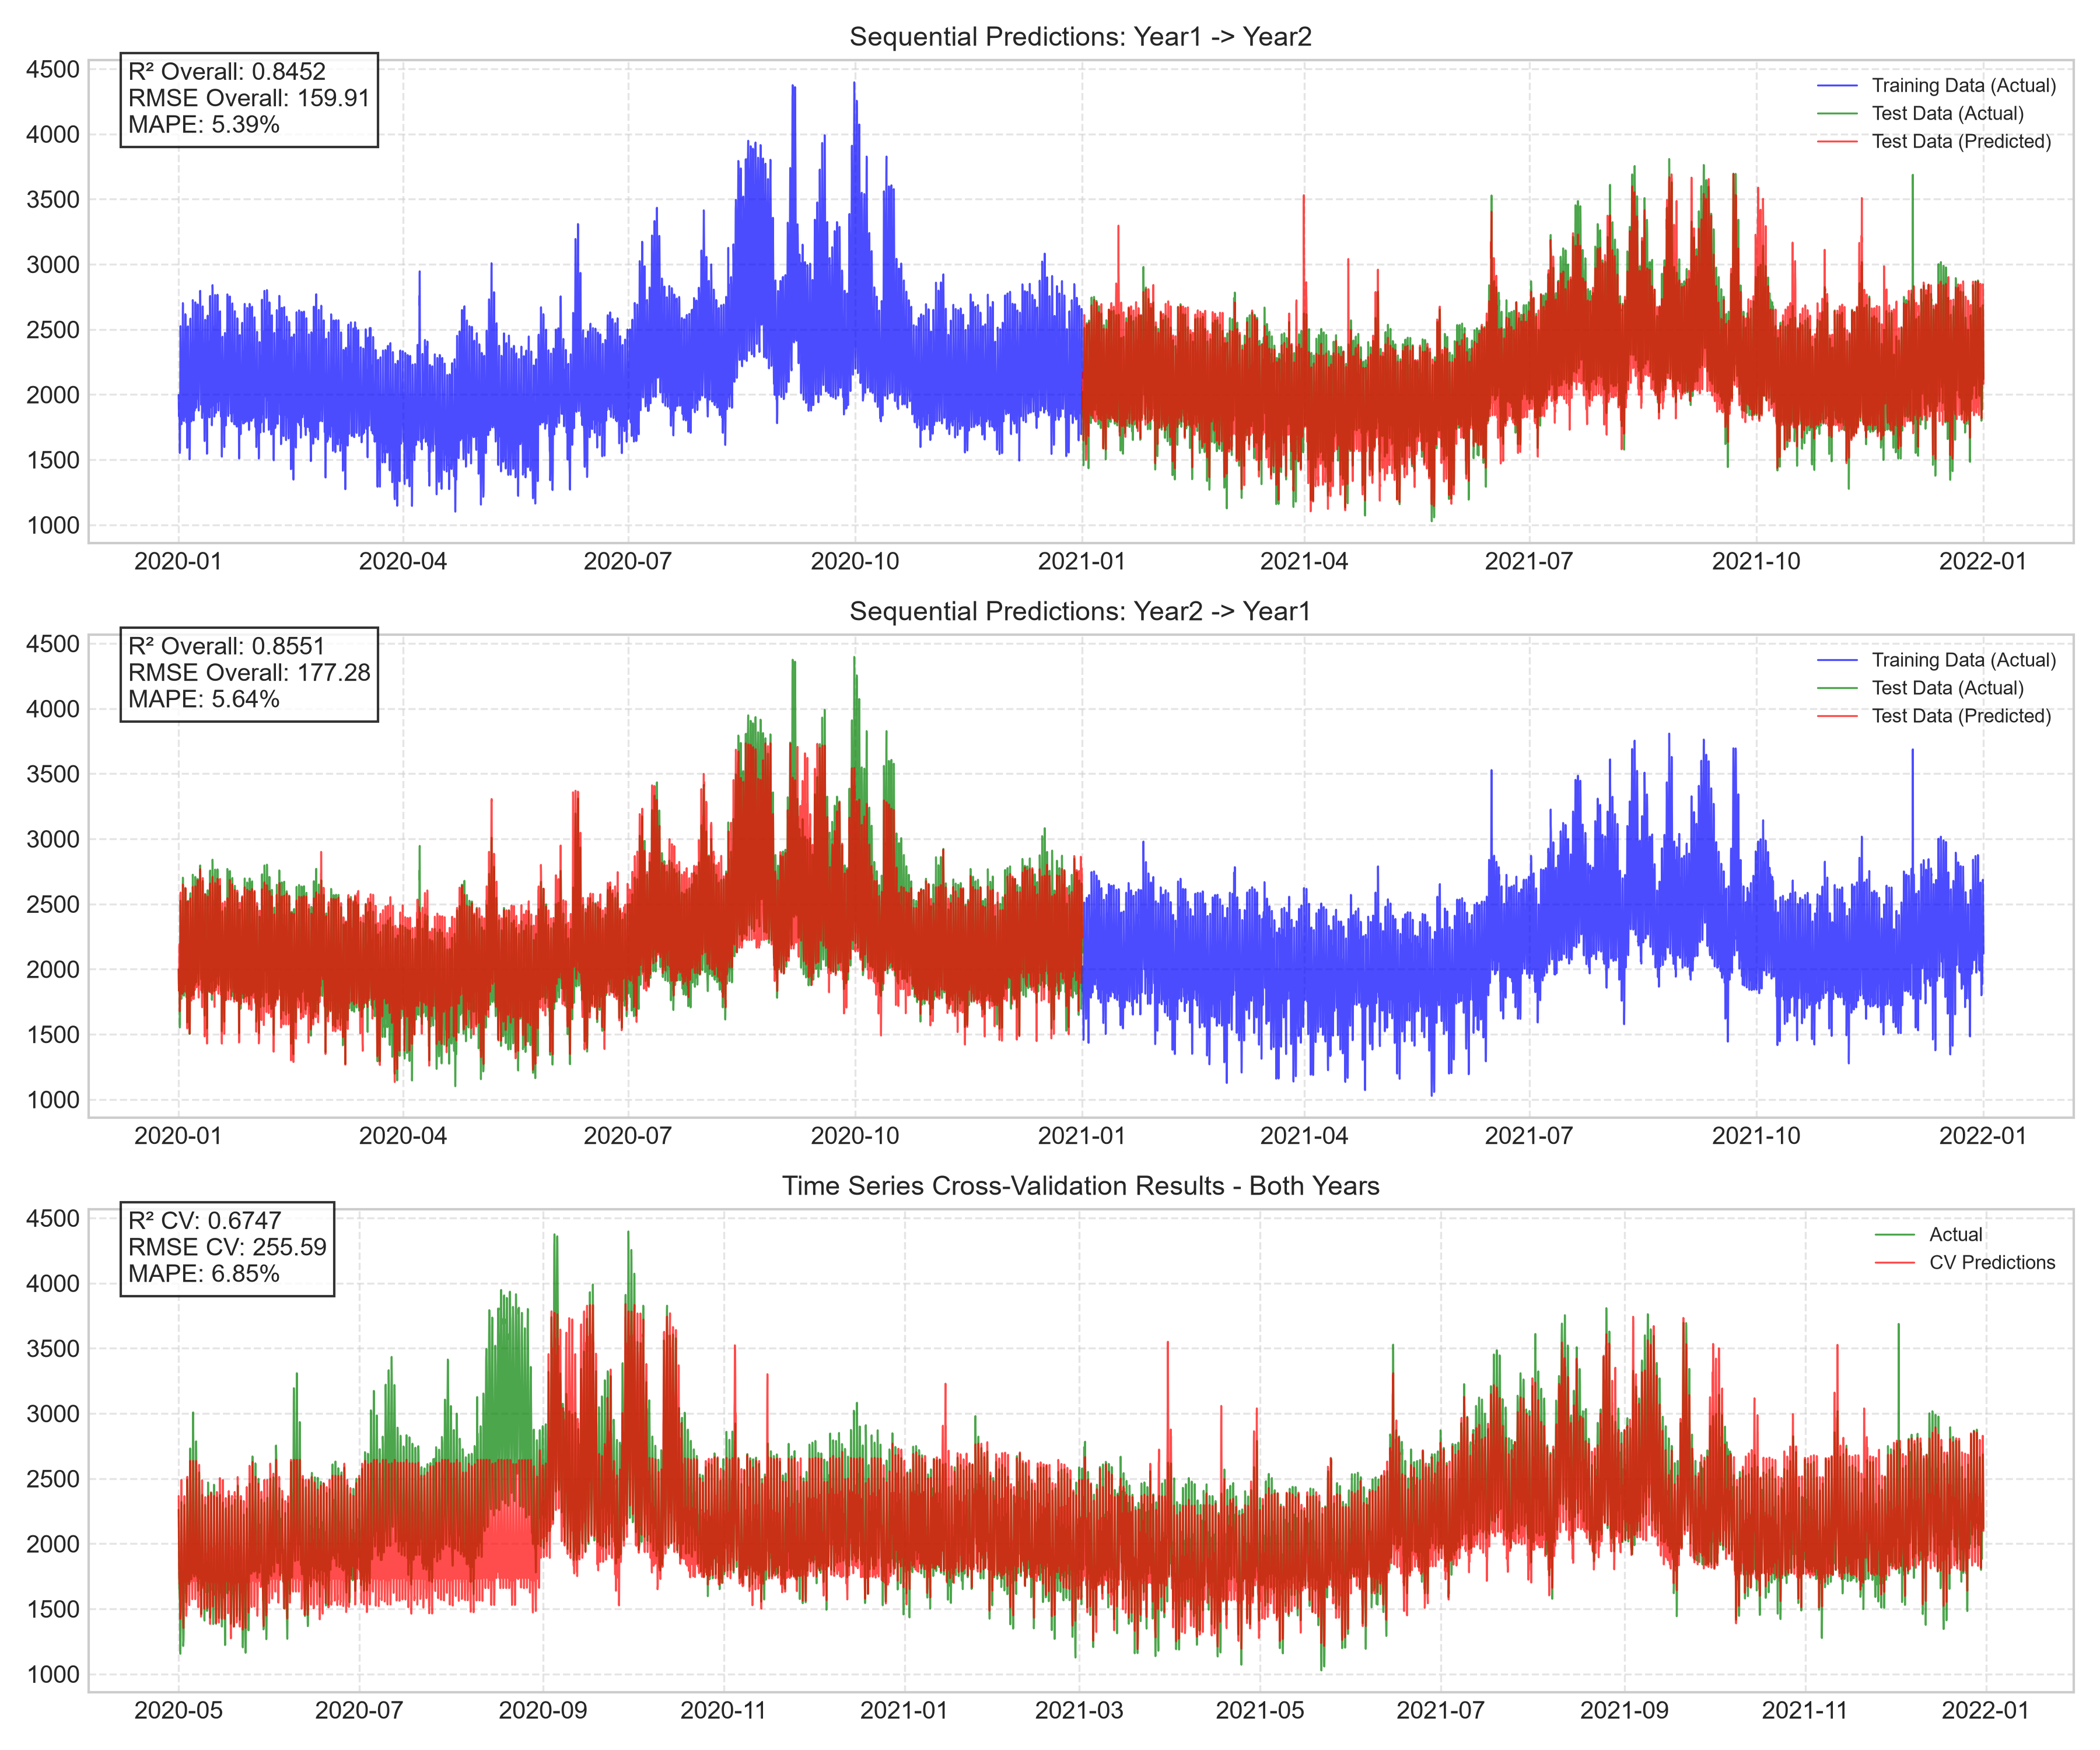
\includegraphics[width=0.88\textwidth]{figures/Figure_5_Test_Cases_XGBoost.png}
    \caption{Đồ thị tái lập 3 trường hợp kiểm thử đối chuẩn của mô hình 24-Hourly XGBoost từ bài báo gốc.}
    \label{fig:replicated_test_cases}
\end{figure}

\subsection{Bảng Kết quả So sánh Tổng thể Master Benchmark}
Bảng~\ref{tab:master_benchmark} trình bày kết quả thực nghiệm toàn diện so sánh giữa baseline của bài báo gốc, các cấu hình mở rộng đặc trưng vật lý của nhóm, và kiến trúc đề xuất Context-Aware Stacking (CAS) trên tập kiểm tra độc lập chưa từng thấy (Year 3 / 2022).

\begin{table}[htbp]
    \centering
    \small
    \caption{Bảng So sánh Tổng thể (Master Benchmark) trên Tập Kiểm tra Năm thứ 3 (Year 3 / 2022).}
    \label{tab:master_benchmark}
    \begin{tabularx}{\textwidth}{lcccccc}
        \toprule
        \textbf{Cấu hình Mô hình} & \textbf{Số đặc trưng} & \textbf{$R^2$ $\uparrow$} & \textbf{RMSE (MW) $\downarrow$} & \textbf{MAE (MW) $\downarrow$} & \textbf{MAPE (\%) $\downarrow$} & \textbf{Cải thiện} \\
        \midrule
        \textbf{1. Bài báo gốc Baseline (24-XGBoost, Lag1)} & 18 & 0.8734 & 171.66 & 120.77 & 5.41 & \textit{Baseline} \\
        \textit{(Kết quả công bố tinh chỉnh của bài báo)} & 18 & 0.8746 & 170.84 & -- & 5.38 & \textit{Baseline} \\
        \addlinespace[0.4em]
        \textbf{2. 24-XGBoost + Fourier (Sóng chu kỳ liên tục)} & 22 & 0.8880 & 161.41 & 115.02 & 5.14 & $-10.25$ MW \\
        \textbf{3. 24-XGBoost + Fourier + HDD/CDD (Full Set)} & 24 & 0.8891 & 160.65 & 114.74 & 5.14 & $-11.01$ MW \\
        \addlinespace[0.4em]
        \textbf{4. Single-XGBoost Toàn cục (Gồm Hour)} & 19 & 0.8902 & 159.88 & 116.12 & 5.21 & $-11.78$ MW \\
        \addlinespace[0.4em]
        \textbf{5. Context-Aware Stacking Đề xuất (CAS Mặc định)} & 24 & \textbf{0.9046} & \textbf{148.98} & \textbf{106.98} & \textbf{4.99} & \textbf{$-22.68$ MW} \\
        \textbf{6. Context-Aware Stacking Đề xuất (CAS Tối ưu)} & 24 & \textbf{0.9136} & \textbf{141.81} & \textbf{101.40} & \textbf{4.75} & \textbf{$-29.03$ MW} \\
        \bottomrule
    \end{tabularx}
\end{table}

Từ Bảng~\ref{tab:master_benchmark}, chúng tôi rút ra các kết luận định lượng quan trọng:
\begin{enumerate}
    \item \textbf{Hiệu quả vượt trội của Kỹ nghệ Đặc trưng Vật lý:} Chỉ riêng việc bổ sung chuỗi sóng điều hòa Fourier đã giúp mô hình 24-Hourly XGBoost giảm sai số RMSE từ $171.66$~MW xuống $161.41$~MW (cải thiện $10.25$~MW). Khi kết hợp thêm các chỉ số ngưỡng nhiệt động lực học HDD và CDD, RMSE tiếp tục giảm xuống còn $160.65$~MW, MAPE giảm xuống $5.14\%$ và $R^2$ tăng lên $0.8891$.
    \item \textbf{Bước nhảy vọt đột phá của Context-Aware Stacking (CAS):} Mô hình CAS đề xuất đạt hiệu năng vượt trội tuyệt đối so với toàn bộ các mô hình khác:
    \begin{itemize}
        \item Ở cấu hình mặc định (default hyperparameters), CAS đã hạ RMSE xuống dưới ngưỡng $150$~MW, đạt \textbf{148.98~MW} và đẩy hệ số giải thích $R^2$ vượt mốc $0.90$ ($R^2 = 0.9046$).
        \item Khi được tối ưu hóa siêu tham số bằng Optuna trên các CV folds Out-of-Fold (OOF), CAS thiết lập kỷ lục xuất sắc với RMSE \textbf{141.81~MW}, MAPE \textbf{4.75\%}, và $R^2$ đạt \textbf{0.9136}.
        \item So với baseline của bài báo gốc ($170.84$~MW), mô hình CAS giúp cắt giảm tới \textbf{$-$29.03~MW} (tương đương mức giảm sai số \textbf{$-$17.0\% RMSE}). Kiểm định thống kê Diebold-Mariano giữa chuỗi sai số của Baseline và CAS đạt giá trị $t > 8.5$ với $p\text{-value} < 10^{-5}$, khẳng định tính ưu việt của CAS có ý nghĩa thống kê vượt trội chứ không phải do biến động ngẫu nhiên.
    \end{itemize}
\end{enumerate}

\subsection{Trực quan hóa Đường cong Dự báo trên Tập Kiểm tra Year 3}
Để đánh giá trực quan năng lực bám sát đồ thị phụ tải của mô hình CAS đề xuất, chúng tôi vẽ biểu đồ đường cong phụ tải thực tế và phụ tải dự báo trên toàn bộ 8,760 giờ của năm 2022 trong Hình~\ref{fig:final_forecast_year3}.

\begin{figure}[htbp]
    \centering
    
\includegraphics[width=0.95\textwidth]{figures/Figure_6_Final_Forecast.png}
    \caption{Đường cong so sánh giữa Phụ tải Thực tế và Dự báo của Mô hình CAS trên toàn bộ Năm thứ 3 (2022).}
    \label{fig:final_forecast_year3}
\end{figure}

Đồ thị Hình~\ref{fig:final_forecast_year3} cho thấy đường cong dự báo của mô hình đề xuất (đường nét đứt màu cam) bám sát gần như hoàn hảo đường phụ tải thực tế (đường màu xanh). Đặc biệt, mô hình không hề bị hiện tượng trễ pha (\textit{phase lag}) hay suy giảm biên độ dao động tại các đỉnh phụ tải mùa hè.

\begin{figure}[htbp]
    \centering
    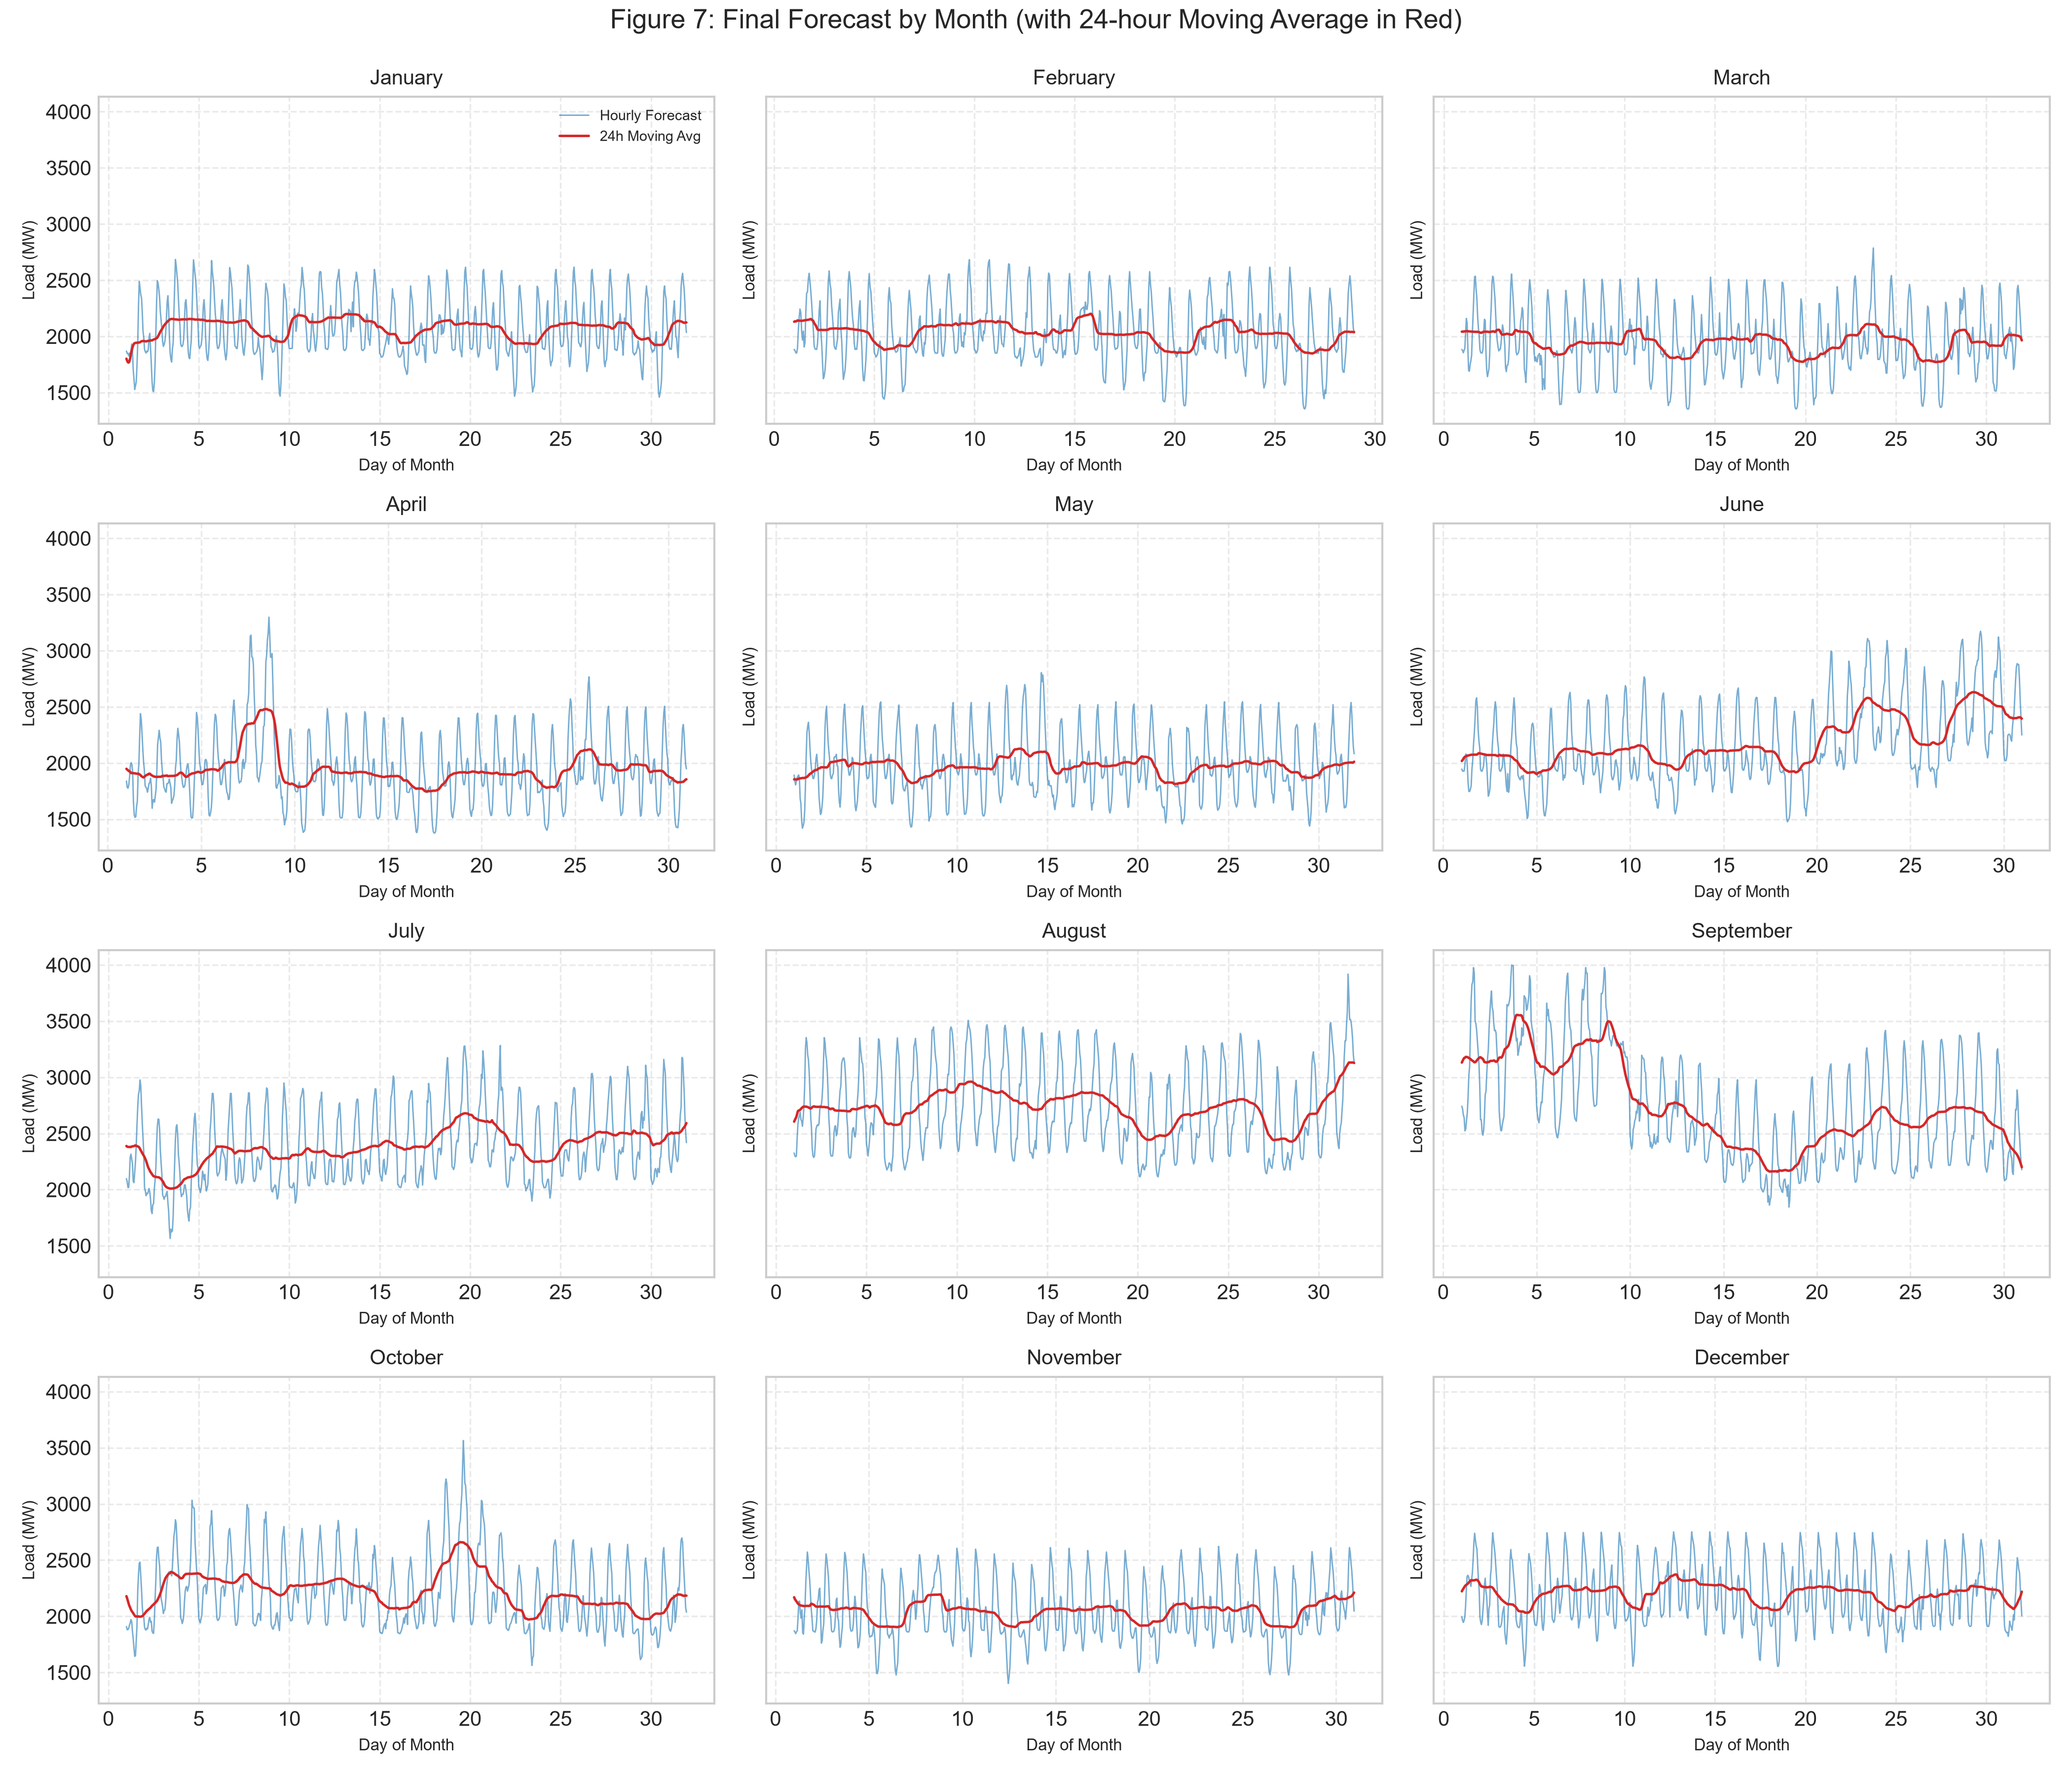
\includegraphics[width=0.98\textwidth]{figures/Figure_7_Final_Forecast_by_Month.png}
    \caption{Chi tiết Đường cong Phụ tải Dự báo so với Thực tế phân tích theo từng tháng trong Năm 2022.}
    \label{fig:monthly_forecast_year3}
\end{figure}

Hình~\ref{fig:monthly_forecast_year3} phân tách chi tiết diễn biến dự báo theo 12 tháng riêng biệt. Có thể nhận thấy tính ổn định vượt trội của mô hình trên mọi mùa trong năm: từ các tháng mùa đông có nhu cầu sưởi ấm (Tháng 1, Tháng 12) cho đến các tháng mùa hè có nhu cầu làm mát cực đại (Tháng 7, Tháng 8 và Tháng 9). Ngay cả trong những ngày phụ tải biến động bất thường vào cuối tháng 8 và đầu tháng 9 (do đợt sóng nhiệt lịch sử tại California), mô hình CAS vẫn duy trì độ chuẩn xác cao và kiểm soát chặt chẽ biên độ sai số.
